\justifying
\NSFCBodyText

\subsubsection{研究内容}

本项目围绕数据对应关系、联合重建机制、约束作用和模式应用四项内容展开。四项内容依次提供训练依据、基础模型、受约束输出和实际应用证据；每一项均对应一条分项技术路线，使用共同的数据划分与评价口径。
% NSFC-ILLUSTRATED BEGIN F02
如图~\ref{fig:framework} 所示，四项研究内容及训练与应用关系。参考资料内开展配对训练，真实CIESM进入独立应用；方法反馈不使用测试集调参。。
\begin{figure}[htbp]
\centering
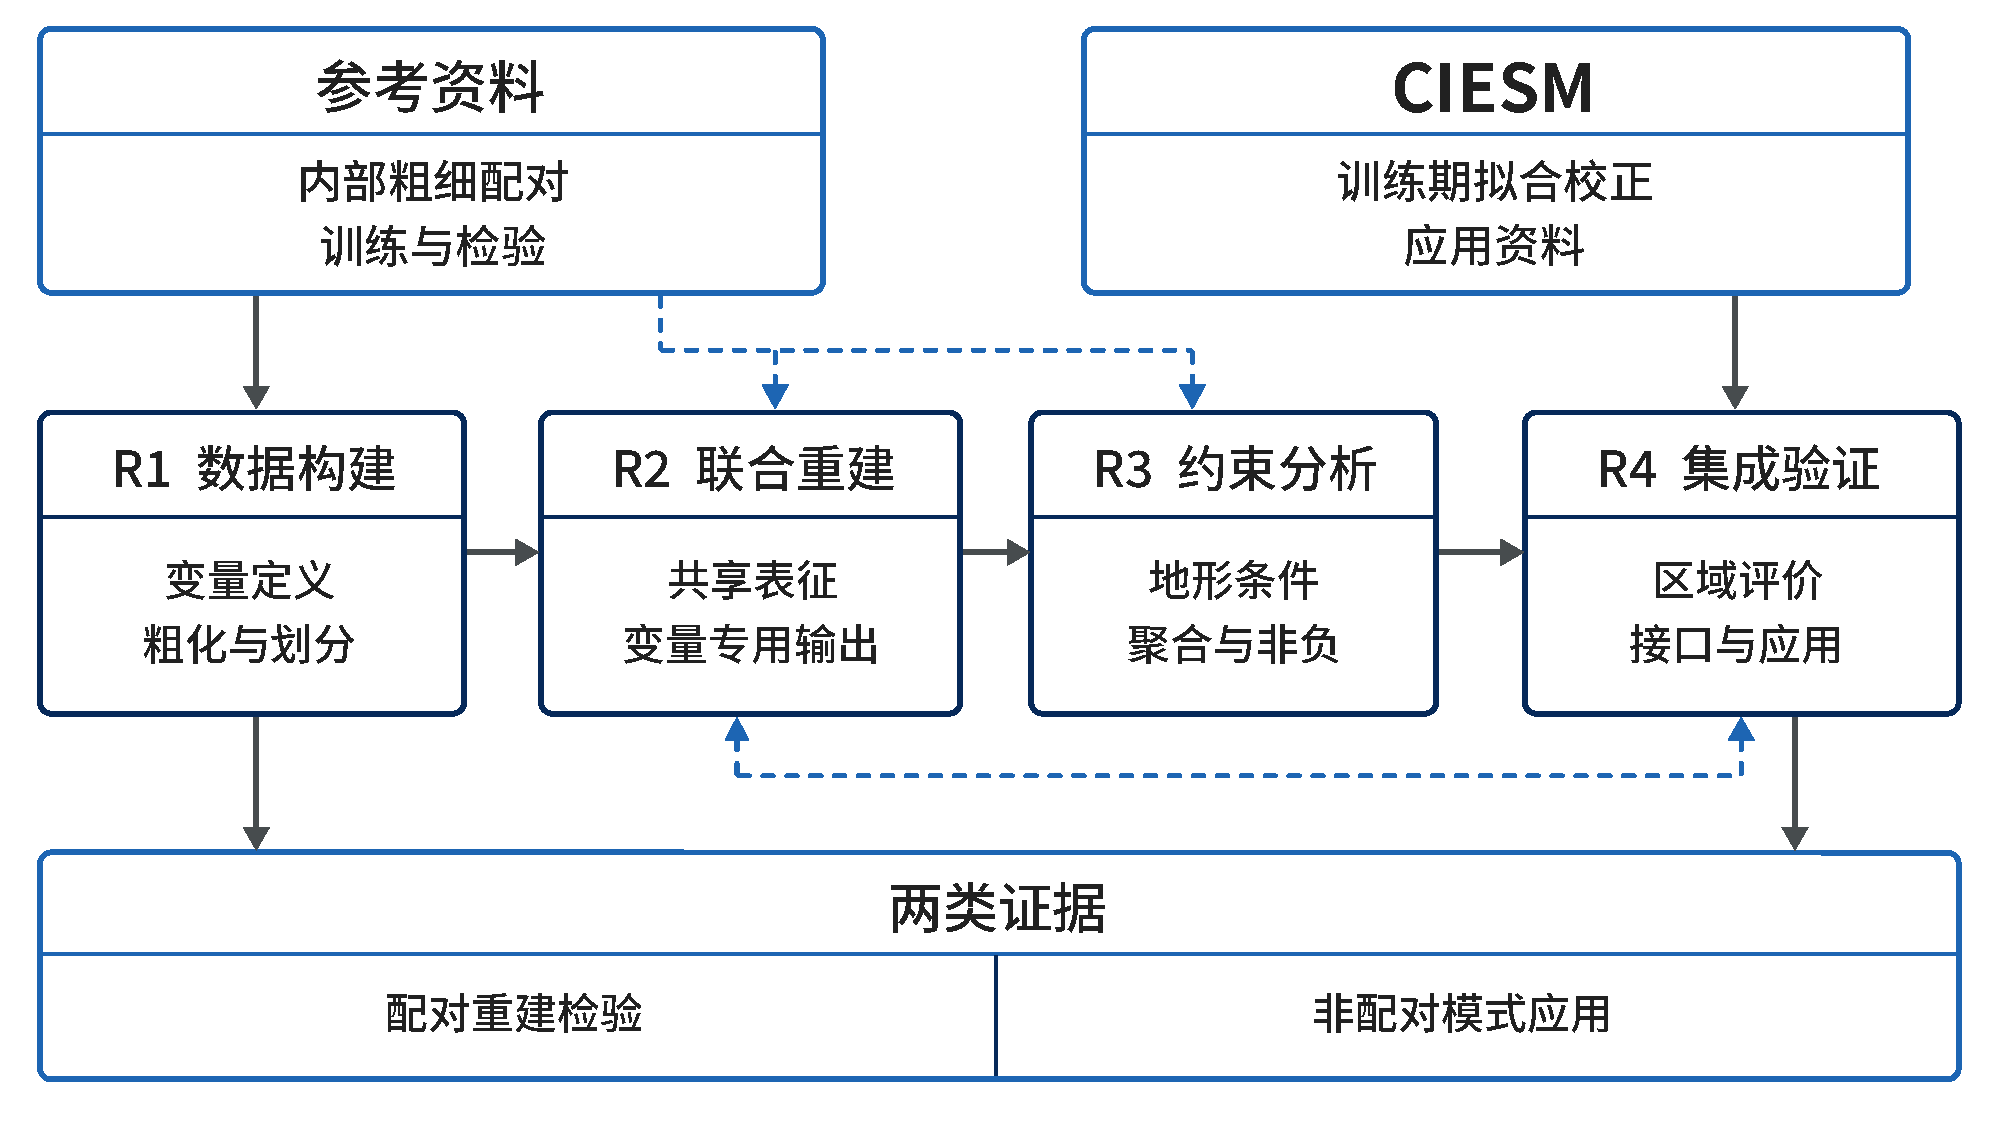
\includegraphics[width=0.95\linewidth]{figures/F02-framework.pdf}
\caption{四项研究内容及训练与应用关系。参考资料内开展配对训练，真实CIESM进入独立应用；方法反馈不使用测试集调参。}
\label{fig:framework}
\end{figure}
% NSFC-ILLUSTRATED END F02


\textbf{研究内容一：CIESM 多源多尺度气象数据构建。}
围绕 CIESM 历史模拟、ERA5、ERA5-Land 及地形资料，辨明变量定义、单位、日历、时间聚合和空间支撑范围。构建再分析资料内部的粗细尺度训练对，并另建 CIESM 非配对应用资料。重点研究不同粗化方式与真实模式输入之间的差异，形成可追溯样本、变量覆盖报告和地形分层，作为后续模型比较的共同基础。

\textbf{研究内容二：多变量多尺度时空超分辨率方法。}
研究气温、风、短波辐射和降水的共同变化及变量特有变化。采用共享时空表征和变量专用输出，比较地形条件下的联合重建与等信息单目标模型。以日尺度空间重建和相邻日的连续性为核心，分析时间上下文是否提供超出单日输入的有效信息，并用条件分布表示无法唯一确定的局地细节。

\textbf{研究内容三：复杂地形引导与物理一致性约束。}
研究地形高程差、坡度、坡向及下垫面条件如何影响局地重建。将粗细网格聚合一致性、非负量约束和变量定义关系与经验性梯度、依赖约束分开。比较不同约束的精度、稳定性和极端保持效应，识别过度约束与域外失效，形成可以逐项检查而非仅靠总损失解释的约束方案。

\textbf{研究内容四：CIESM 集成与区域应用验证。}
将前三项产出整理为 CIESM 区域数据增强模块，开展公开资料兼容性验证，并在获得实验室接口资料后进行联调。围绕新疆典型地形单元、连续独立时段和跨区域样本，评价平均状态、空间结构、时间连续性、联合分布与极端事件。以可复现实验记录、接口运行结果及实际应用证据支撑成果验收。

\subsubsection{研究目标}

总体目标是形成一套面向新疆复杂地形、能够解释粗细尺度关系的 CIESM 多变量气象场增强方法，给出其精度收益、约束效果及适用边界。课题的预期成果包括算法、区域试验数据和可复现评估流程，论文与集成应用成果按 P02 方向要求组织。

数据层面，形成覆盖四类关键变量的来源与处理记录，明确可用时间频率、目标网格和共同陆地区域；模型层面，在同等输入和计算预算下比较独立重建与联合重建；约束层面，报告每个变量的聚合残差和非法输出比例，并分析结构与极端指标的变化；应用层面，完成从 CIESM 文件读入到高分辨率输出、粗化复核和应用示例的完整运行。

研究设计暂以\textbf{【暂定 0.1°日尺度区域网格】}作为共同目标，以资料内部配对实验的地形分层空间结构误差作为唯一主要评价量，以跨变量秩相关矩阵误差作为关键次要评价量。主次评价量的定义、汇总权重及对照模型在验证集上确定后固定，独立测试集仅用于最终估计。期望观察到方向一致且跨重复实验稳定的改善；不将任意百分比预设为已经取得或必然达到的效果。

\subsubsection{拟解决的关键科学问题}

\textbf{其一，粗细尺度关系在何种条件下可迁移？}
再分析场内部配对能够提供训练目标，真实 CIESM 则带有不同的偏差与天气轨迹。需要辨明空间粗化、季节背景和输入分布差异对重建的影响，并确定数据校正后仍能保留和验证的气候信息。

\textbf{其二，地形条件如何改变变量共享的收益？}
温度、风、辐射和降水对地形和天气条件的响应不同。共享表征可能利用相关信息，也可能使高方差变量主导优化。需要在等信息独立基线下判断联合训练的增益，考察其是否随地形、季节和极端样本而改变。

\textbf{其三，一致性约束怎样影响有效细节？}
严格匹配聚合量并不自动保证所有细节正确；软性梯度和依赖关系也可能限制真实异常。需要区分约束带来的数学一致性和独立样本上的气象合理性，分析收益及代价，并给出约束失效时的简化方案。

\subsubsection{研究方法}

\textbf{（1）资料选择、样本构造与验证划分。}
对每项 CIESM 数据记录模式版本、试验名、成员、网格、频率和文件校验值。拟使用公开 historical 资料与同期再分析的共同覆盖期，优先核对近地面气温、近地面风、地表向下短波辐射和降水；变量在实际文件中的名称及统计意义以元数据为准。风场优先保留东西、南北分量；若只有风速，则仅开展标量风速任务，单独说明不能评价风向和向量关系。

训练、验证和测试采用连续年份划分，初步设置为\textbf{【暂定训练期 1981—2005 年、验证期 2006—2009 年、测试期 2010—2014 年】}，最终取实际共同覆盖期。先划分原始时间和区域，再估计标准化、偏差校正、地形统计与阈值，避免同一过程的相邻样本进入不同集合。使用时间窗口时在集合边界留出不少于半个窗口长度的间隔；空间小块按完整地形区域分组，训练增强不跨入留出区域。

以高分辨率参考场 $Y$ 构造粗化算子 $A$，形成 $(AY,Y)$ 训练对，并使 $A$ 尽量反映 CIESM 网格的面积与采样方式。ERA5-Land 可作为有明确来源说明的细网格参考，但对原始强迫主要经插值获得的变量，另设仅插值对照，识别网络是否只是重现插值纹理。ERA5 的同日粗场可作为额外条件，但仅选用在 CIESM 中具有同定义、同频率对应项的变量；应用时无法获得的条件不进入主模型训练。它与目标参考的资料关系在记录中保留。真实 CIESM 样本 $X$ 不与 $Y$ 按日期计算配对误差，而在季节分布、空间统计和尺度残差层面评价。

气温统一单位后处理；降水率先依据时间边界积分为相应时段量，辐射累计量按实际累计区间换算。逐一核对闰日、不同日历、累计起点与时区，禁止将累计值直接当瞬时值。目标陆地掩膜与粗细网格共同覆盖范围共同决定面积权重；只有覆盖完整、权重定义成立的粗网格参与严格聚合比较，边界与缺测网格另行报告。
% NSFC-ILLUSTRATED BEGIN F03
如图~\ref{fig:data} 所示，数据构建与样本隔离路线。两类资料分别组织；训练、验证、测试是共同划分约定，不表示资料来源与集合的一一对应。。
\begin{figure}[htbp]
\centering
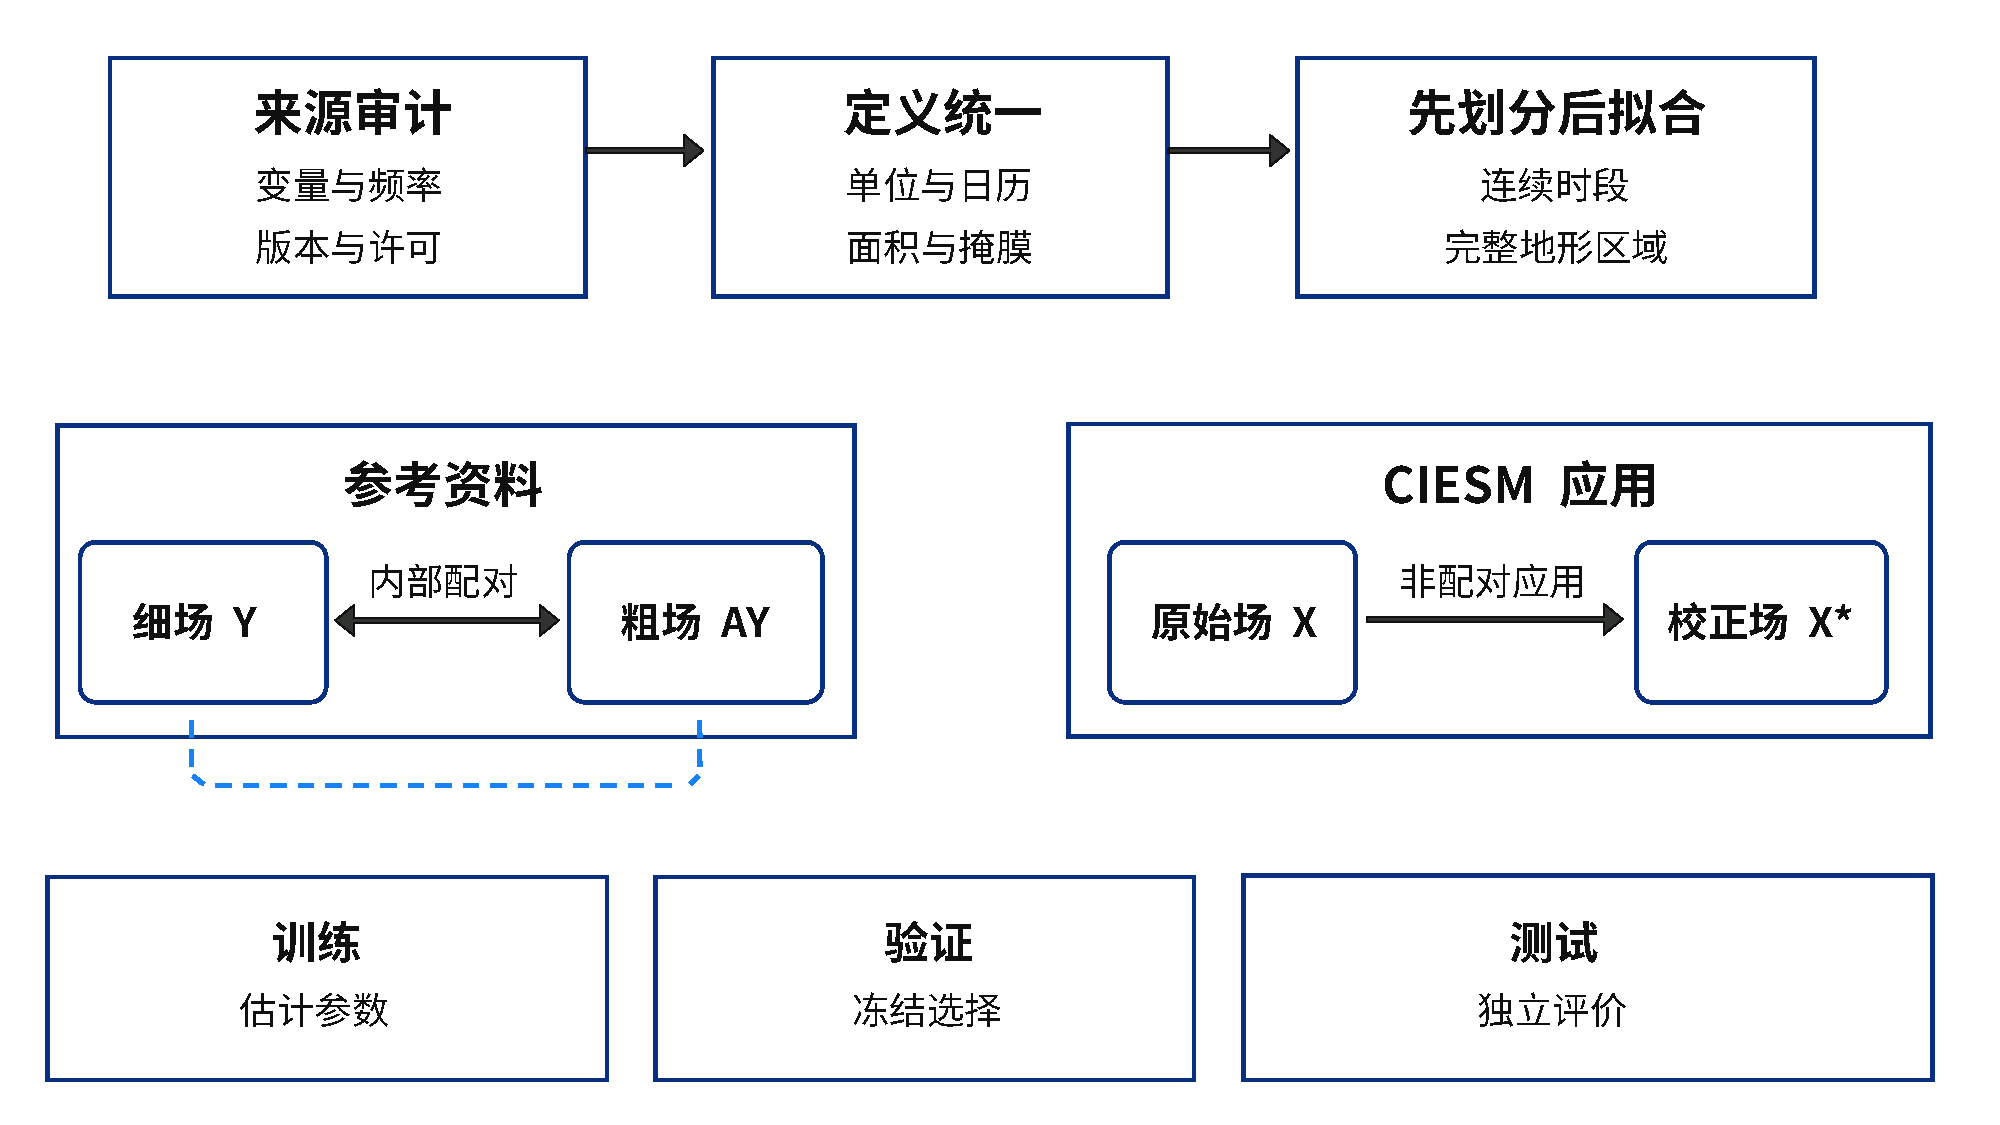
\includegraphics[width=0.95\linewidth]{figures/F03-data.pdf}
\caption{数据构建与样本隔离路线。两类资料分别组织；训练、验证、测试是共同划分约定，不表示资料来源与集合的一一对应。}
\label{fig:data}
\end{figure}
% NSFC-ILLUSTRATED END F03


\textbf{（2）分布校正与时空联合重建。}
对 CIESM 输入先应用在训练期估计的分布变换 $B$，得到目标大尺度状态 $X^{\star}=B(X)$。$B$ 以训练期参考资料经 $A$ 粗化后的分布为校正目标，使应用条件与训练条件的变量定义和尺度支撑一致；参考训练分支直接使用 $AY$。基线包含不校正、逐变量分位数校正和适当的趋势保持校正；多变量统计校正作为强化对照，选择依据为验证集上的边缘分布与依赖表现\cite{Lange2019ISIMIP,Cannon2018MBCn}。推断期不得用测试目标重新拟合 $B$。跨时期变化同时报告原始 $X$、校正后 $X^{\star}$ 和重建场的统计差异，避免把校正后的信号误称为原模式信号原样保留。

模型写为
\begin{equation}
\widetilde{Y}_{t}=G_{\theta}\bigl(X^{\star}_{t-k:t+k},Z,S_t,\xi\bigr),
\end{equation}
其中 $Z$ 表示地形和下垫面条件，$S_t$ 为季节或日序信息，$\xi$ 为可选随机变量。核心模型先学习条件中心场，再检验小规模随机残差是否能改善概率校准和空间分布。由于应用是离线气候资料重建，时间窗口可使用前后邻日；这一设置不解释为实时预测能力。

采用多尺度卷积或轻量时序模块表征缓慢变化背景与局地残差，设置变量专用输出和按训练资料尺度归一的损失权重。气温和风的连续误差、降水发生与正降水量的间歇性分别建模。降水零值频率及极端尾部由独立评价确认，不通过视觉平滑程度判断。时间上下文以\textbf{【暂定连续 7 日窗口】}起步，并与单日、打乱邻日顺序和缩短窗口对照，以辨别相邻时刻本身是否提供有效信息。

对照采用逐级设计：面积一致的插值；统计偏差校正加插值；等输入的独立单目标模型；共享表征的联合模型；联合模型加地形；加入显式一致性条件的完整模型。独立单目标模型也读取与联合模型相同的多变量粗场及地形条件，总参数量级和训练预算控制一致，另以传统仅单变量输入模型作应用参照。由此将“可利用的信息更多”与“联合训练方式更有效”分开解释。对共享与独立、有地形与无地形进行两因素对照；各组使用相同校正和相同投影规则，并检验地形与共享的交互效应。若只有共享主效应成立，则结论限于共享学习收益；只有交互得到支持，才解释为地形信息增强了该收益。
% NSFC-ILLUSTRATED BEGIN F04
如图~\ref{fig:reconstruction} 所示，多变量时空重建与等信息对照。共享表征连接四类专用输出，随机残差为条件性扩展，独立基线保持同信息和总预算。。
\begin{figure}[htbp]
\centering
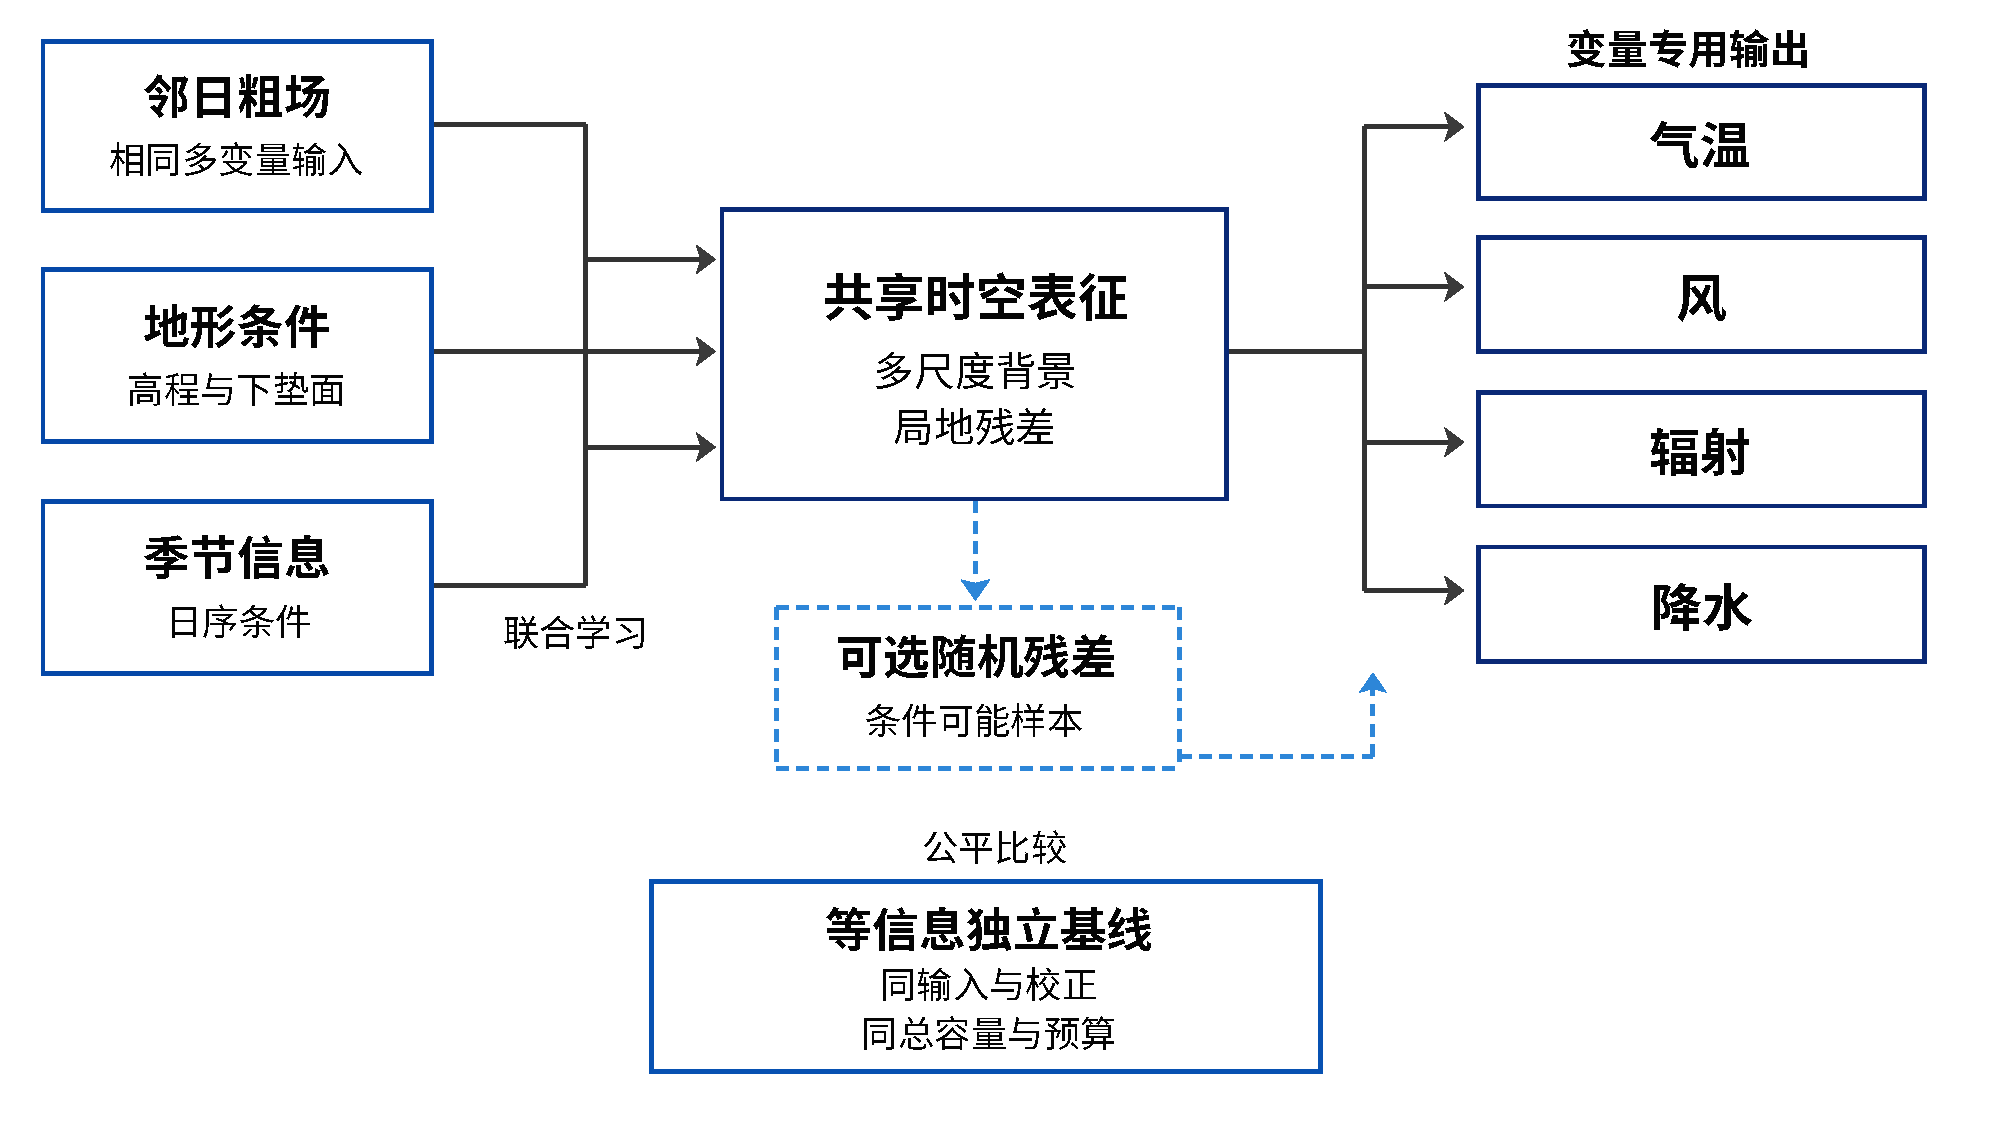
\includegraphics[width=0.95\linewidth]{figures/F04-reconstruction.pdf}
\caption{多变量时空重建与等信息对照。共享表征连接四类专用输出，随机残差为条件性扩展，独立基线保持同信息和总预算。}
\label{fig:reconstruction}
\end{figure}
% NSFC-ILLUSTRATED END F04


\textbf{（3）可定义的硬约束和待验证的软约束。}
设粗网格 $c$ 内细网格面积权重为 $w_{ci}$，满足共同有效覆盖范围内 $\sum_iw_{ci}=1$。对可使用有符号残差的连续变量，先研究约束投影
\begin{equation}
\widehat{Y}=\underset{y}{\arg\min}\;\|y-\widetilde{Y}\|_{W}^{2},
\qquad \text{满足}\quad Ay=X^{\star},
\end{equation}
其中 $W$ 为正定权重矩阵，$A$ 为冻结的聚合算子。对于一般非嵌套网格，先验证约束可行性、算子秩和数值条件，不直接沿用整齐像素块的均值修正。实际投影残差逐网格输出，作为实现正确性的检查项。

对嵌套网格中的非负降水，可将非负细节权重 $q_i$ 按粗格总量归一：
\begin{equation}
\widehat{P}_i=P_c^{\star}\frac{q_i}{\sum_{j\in c}w_{cj}q_j}.
\end{equation}
此式要求 $P_c^{\star}\geq0$ 且分母为正。粗格为零时全部细格置零；分母退化时使用可记录的非负均匀分配，不通过无说明的常数扰动改变总量。降水发生掩膜与正值权重分开，防止把少数湿格扩散为普遍毛毛雨。非嵌套网格采用带非负条件的数值投影，并检查其可行性。短波辐射也实施非负和相应时段聚合检查。

若输入含风分量，先核对分量与风速的统计时段。日均风分量的模长仅称为“日均风矢量模长”，不能当作日平均风速；只有同一瞬时分辨率的分量才先合成风速再按日聚合。仅有日平均标量风速时独立建模，不添加由日均分量强推标量风速的约束。以上条件属于变量定义或选定聚合关系的一致性。由于本课题未同时包含蒸发、储水、辐射净收支及所有热通量，不将这些条件表述为完整的水量、能量或动量守恒。

地形引导通过原生模式地形与细网格高程差、地形起伏、坡度坡向及陆面类别进入条件分支。温度随高程变化的关系按季节与地形分层估计，并允许逆温等例外；空间梯度和变量相关性使用软惩罚，权重仅由验证集选择。将软约束权重从零逐步增加，观察主次评价量、极端分位数和物理范围异常率的共同变化，保留收益与代价曲线，不只报告最优单点。
% NSFC-ILLUSTRATED BEGIN F05
如图~\ref{fig:constraints} 所示，显式一致性与经验约束的作用区分。聚合、非负和变量定义条件逐项检查，数值一致性与独立样本收益分别评价。。
\begin{figure}[htbp]
\centering
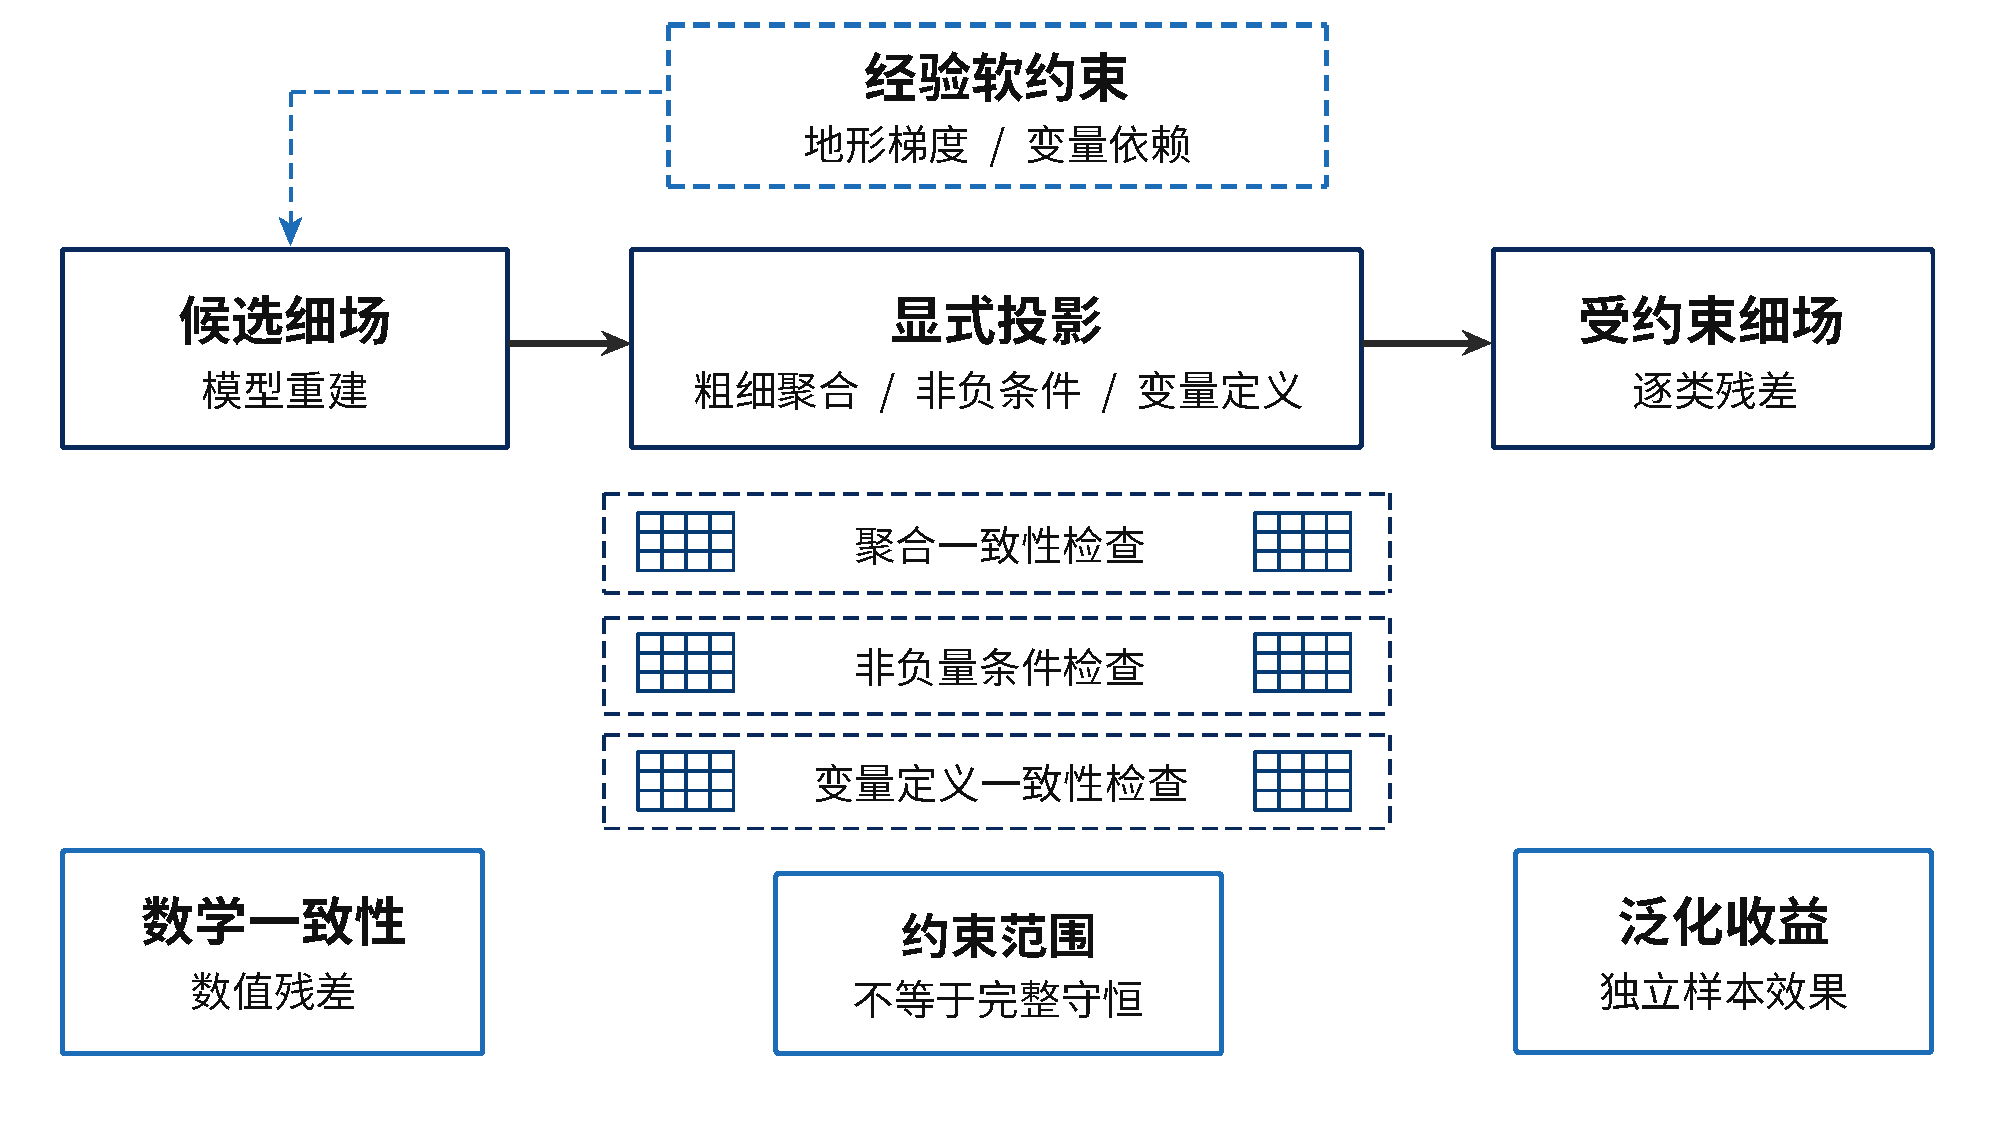
\includegraphics[width=0.95\linewidth]{figures/F05-constraints.pdf}
\caption{显式一致性与经验约束的作用区分。聚合、非负和变量定义条件逐项检查，数值一致性与独立样本收益分别评价。}
\label{fig:constraints}
\end{figure}
% NSFC-ILLUSTRATED END F05


\textbf{（4）多层评价与统计证据。}
在再分析内部配对实验中，报告按面积和训练期尺度归一的平均绝对误差、均方根误差及异常相关，并分温度、风、辐射和降水列示。空间结构主要评价量采用地形分层半变异函数差异的归一化积分，积分以预定距离档位加权求和近似，归一化尺度取训练期参考半变异幅度；近常数分层采用预先固定的正尺度下限并单列标识，避免除零及异常放大。距离档位和变量权重在训练、验证资料中固定；跨变量依赖的关键次要评价量采用去季节、训练尺度标准化后的变量秩相关矩阵误差。两者都在同一测试样本上与等信息独立基线比较。另按变量设置平均误差非退化界限，界限依据验证资料的误差尺度预先固定；主要指标改善但任一变量越过该界限时，不判为四变量方案整体有效。在查看测试结果前，依据验证资料的误差尺度确定最小有意义增益并记录。定义增益为独立基线误差减去本方法误差，以正值表示改善。其区间上界低于最小有意义增益时，不支持有效增益假设；区间下界高于该阈值且逐变量非退化条件均通过时，才判为支持；跨越阈值时报告证据不足。

补充评价包括功率谱、邻日自相关、湿日频率、强降水分位数、持续高温及大风事件统计。复合条件从四类变量能够直接定义的组合中选择，以训练期分位数固定阈值，在测试期评价共同发生频率；不引入未收集的湿度等变量来定义事件。采用\textbf{【暂定训练期第 95 百分位作为高值事件阈值、降水 1 毫米/日作为湿日阈值】}，并进行阈值敏感性分析。事件持续天数以完整日序列计算，缺测中断不拼接。

主要地形单元包括天山及南北坡、准噶尔盆地和塔里木盆地，按独立的数字高程模型（DEM）和地理范围划定。在空间留出试验中，每次使用完整区域作外部检验，不通过邻近重叠小块泄漏其目标信息。另设置\textbf{【暂定河西走廊—祁连山地区】}作为跨区域检验，地理边界与训练缓冲区在取数时固定。跨区域结果反映迁移能力，不用于回调主测试集的模型选择。

随机模型报告连续排序概率评分、区间覆盖及区间宽度，以训练期气候分布和确定性模型构造的简单残差集合作为对照。核心方法拟采用\textbf{【暂定 3 次独立随机种子、按年份与事件块重抽样形成 95\% 置信区间】}；随机种子用于报告训练波动，统计推断以时空块为单位，避免将种子数或高度相关格点当作独立气候样本数。独立年份较少时同时展示逐年结果。主要指标用于检验核心假说；次要及分层指标用于解释，如开展多项推断则报告多重比较处理；不将个别分层的改善推广为全区域结论。

真实 CIESM 端分别比较原始场、校正场和增强场的季节均值、分位数、空间谱及联合统计，并检验增强场聚合至 $X^{\star}$ 的残差。再分析一致性是参考资料内的证据；若获得具有使用权限且未参与训练的站点或独立产品，则按其空间代表性另行核验。ERA5 与 ERA5-Land 的相互比较不计作独立观测验证。

\subsubsection{技术路线}

\textbf{总体技术路线。}
首先由多源资料构建产生统一变量、时空划分和粗化算子；这些产物固定后，第二项研究建立多变量时空重建模型，第三项研究在同一模型与样本上加入地形条件及逐类约束，第四项研究使用选定算法处理 CIESM 文件并开展区域与接口验证。参考资料进入训练和评估分支，真实 CIESM 进入训练期限定的分布校正及应用分支；两者在经过定义明确的粗尺度条件变换后衔接，不将原始模拟日与参考日强行配对。四项研究共享版本化的数据记录，验证问题可以反馈为模型修正，但测试集不参与调参。

\textbf{面向研究内容一的数据构建路线。}
输入为公开 CIESM、ERA5、ERA5-Land、DEM 和土地覆盖资料。依次核验变量及时间频率、转换单位和日历、固定有效覆盖区域、划分时段与地形，再由参考资料构造粗细训练对；同时保留独立的 CIESM 应用样本。输出为样本索引、可复现预处理程序与资料差异说明。通过抽样手工复核、粗化复算和训练测试隔离检查验证数据可靠性；冻结后的样本和算子进入联合建模与约束研究。

\textbf{面向研究内容二的联合重建路线。}
输入为粗细训练对、统一地形条件和相邻时刻信息。先拟合可解释的统计与插值对照，再训练等信息独立模型和共享表征模型，最后按验证结果选择是否加入随机残差。输出为条件中心场、可选样本集合及训练配置。以空间结构主要评价量、依赖次要评价量及时间顺序对照检验联合与时间信息的贡献；固定的候选模型作为约束分析的共同起点。

\textbf{面向研究内容三的约束分析路线。}
输入为候选重建场、面积聚合算子和地形分层。先实施数学上可检查的非负、聚合与变量定义关系，再逐项加入地形梯度和依赖软约束，比较不同强度下的结构、极端与不一致残差。输出为受约束场、逐类残差及失效条件。通过等预算消融、干湿分层和约束冲突诊断验证机制；具有明确收益及适用范围的配置进入 CIESM 应用。

\textbf{面向研究内容四的集成验证路线。}
输入为选定模型、真实 CIESM 文件与固定测试区域。先按公开数据完成读入、分块推断、细网格输出和粗化复核，再依据实验室提供的实际接口进行联调，记录运行环境、资源消耗和输出语义。输出为算法模块、区域试验数据和应用示例。公开格式兼容性、实验室联调成功及正式成果接收分别保留证据；只有取得相应实际记录，才报告相应层级的集成完成。
% NSFC-ILLUSTRATED BEGIN F06
如图~\ref{fig:integration} 所示，CIESM集成与应用证据路线。公开兼容性、实验室联调、实际应用与接收均按真实记录确认，图示为拟开展流程。。
\begin{figure}[htbp]
\centering
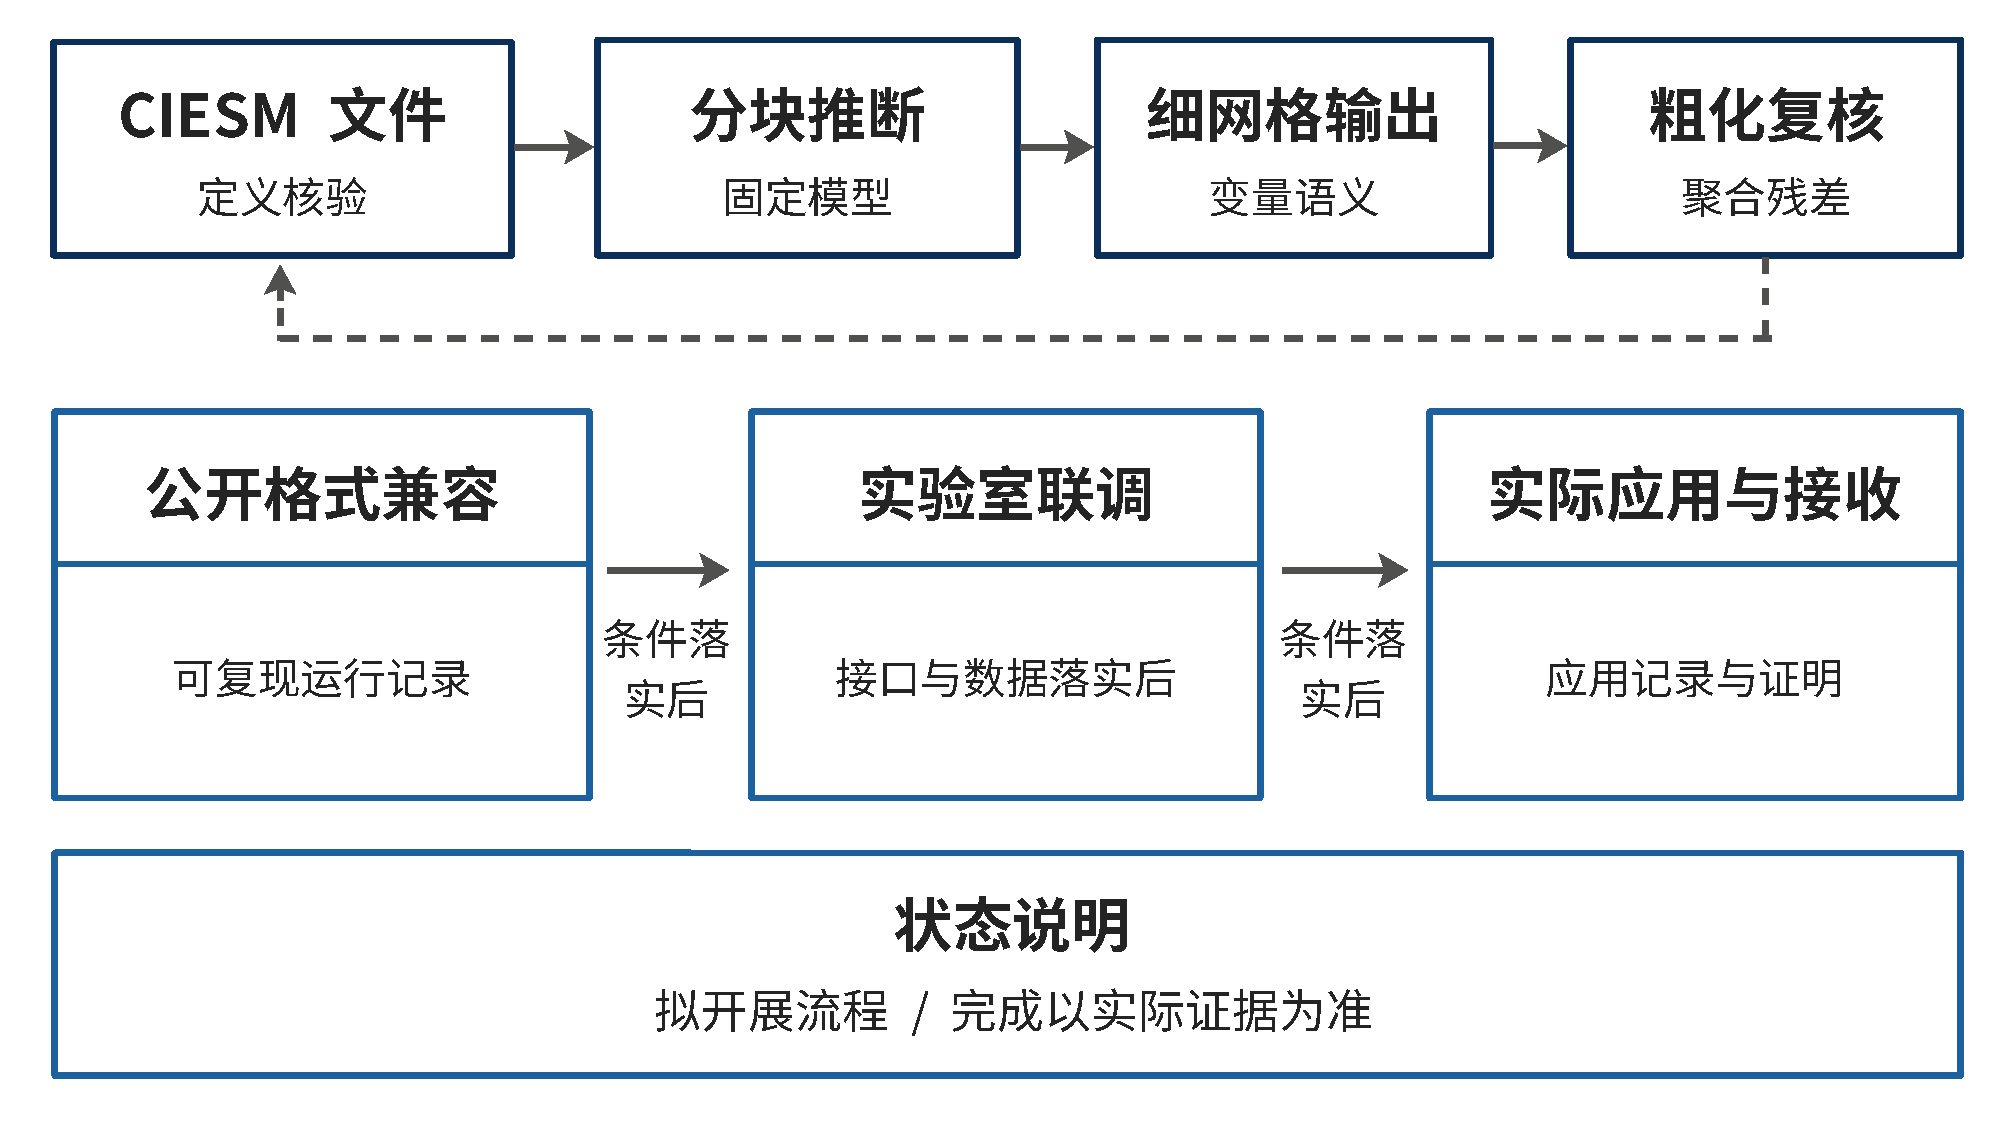
\includegraphics[width=0.95\linewidth]{figures/F06-integration.pdf}
\caption{CIESM集成与应用证据路线。公开兼容性、实验室联调、实际应用与接收均按真实记录确认，图示为拟开展流程。}
\label{fig:integration}
\end{figure}
% NSFC-ILLUSTRATED END F06


为保留题目中的时间增强研究，另设条件性的小规模日内试验：在已取得高频参考场、核心日尺度结果稳定且实验室输入频率允许时，研究\textbf{【暂定由日尺度条件生成 6 小时统计一致的子时段序列】}。以参考资料自身聚合构造训练对，保持子时段量回聚合为对应日量，加入日序和当地太阳时间条件，并以概率校准、日内变化和极端时段分布检验。其输出是条件可能序列，不解释为已知真实日内轨迹。该扩展单独报告，不能替代日尺度四变量核心任务。

\subsubsection{关键技术}

第一项关键技术是对真实模式网格、变量统计时段与参考资料建立可复算的聚合关系。它决定训练对是否成立及约束是否有意义，处理次序必须先于网络复杂化。重点核验累计量、不同日历、边界掩膜与非嵌套网格，避免将数据处理误差误判为模型偏差。

第二项关键技术是控制联合学习中的负迁移。保持等信息单目标基线，以变量专用分支、训练尺度归一与适度共享进行比较；若某变量的收益持续不稳定，保留其独立输出路径，并报告这一结果所揭示的共享边界，而不以其他变量的平均收益掩盖退化。

第三项关键技术是把约束可行性与泛化收益分开验证。数值实现先检查是否满足给定条件，随后用独立样本比较是否改善重建。约束冲突或参考场不支持时，停用相应软约束，保留可证明成立的部分，同时说明被舍弃条件及其影响。

\subsubsection{可行性分析}

课题以公开模式资料和再分析为起点，采用已有统计降尺度、卷积重建与约束投影作为可复现对照，方法实施具有清晰基础。申请人在多尺度时间序列建模方面的研究积累，可支持时空信息组织和实验设计；现有 GPU 与软件环境可支持区域分块训练，具体研究基础和工作条件见第三部分。

主要不确定性是公开 CIESM 四类变量的共同时间频率、参考资料的独立信息以及实验室接口落实。项目在第一季度完成资料审计并联系接口，不等待复杂模型完成后再确定应用条件。若关键变量仅有月资料，则以月尺度分布与空间重建作为阶段成果，同时明确日尺度核心验证尚未完成；在取得合适高频数据前不报告日极端或日内增强达标。若生成模型成本超过计划，则优先完成确定性联合模型、约束消融和接口验证，保留概率扩展为后续研究。
% NSFC-ILLUSTRATED BEGIN F07
如图~\ref{fig:evaluation} 所示，公平消融与两类验证证据。矩阵表示四种拟比较配置；两类资料使用各自评价口径，结论同时检查非退化及不确定性。。
\begin{figure}[htbp]
\centering
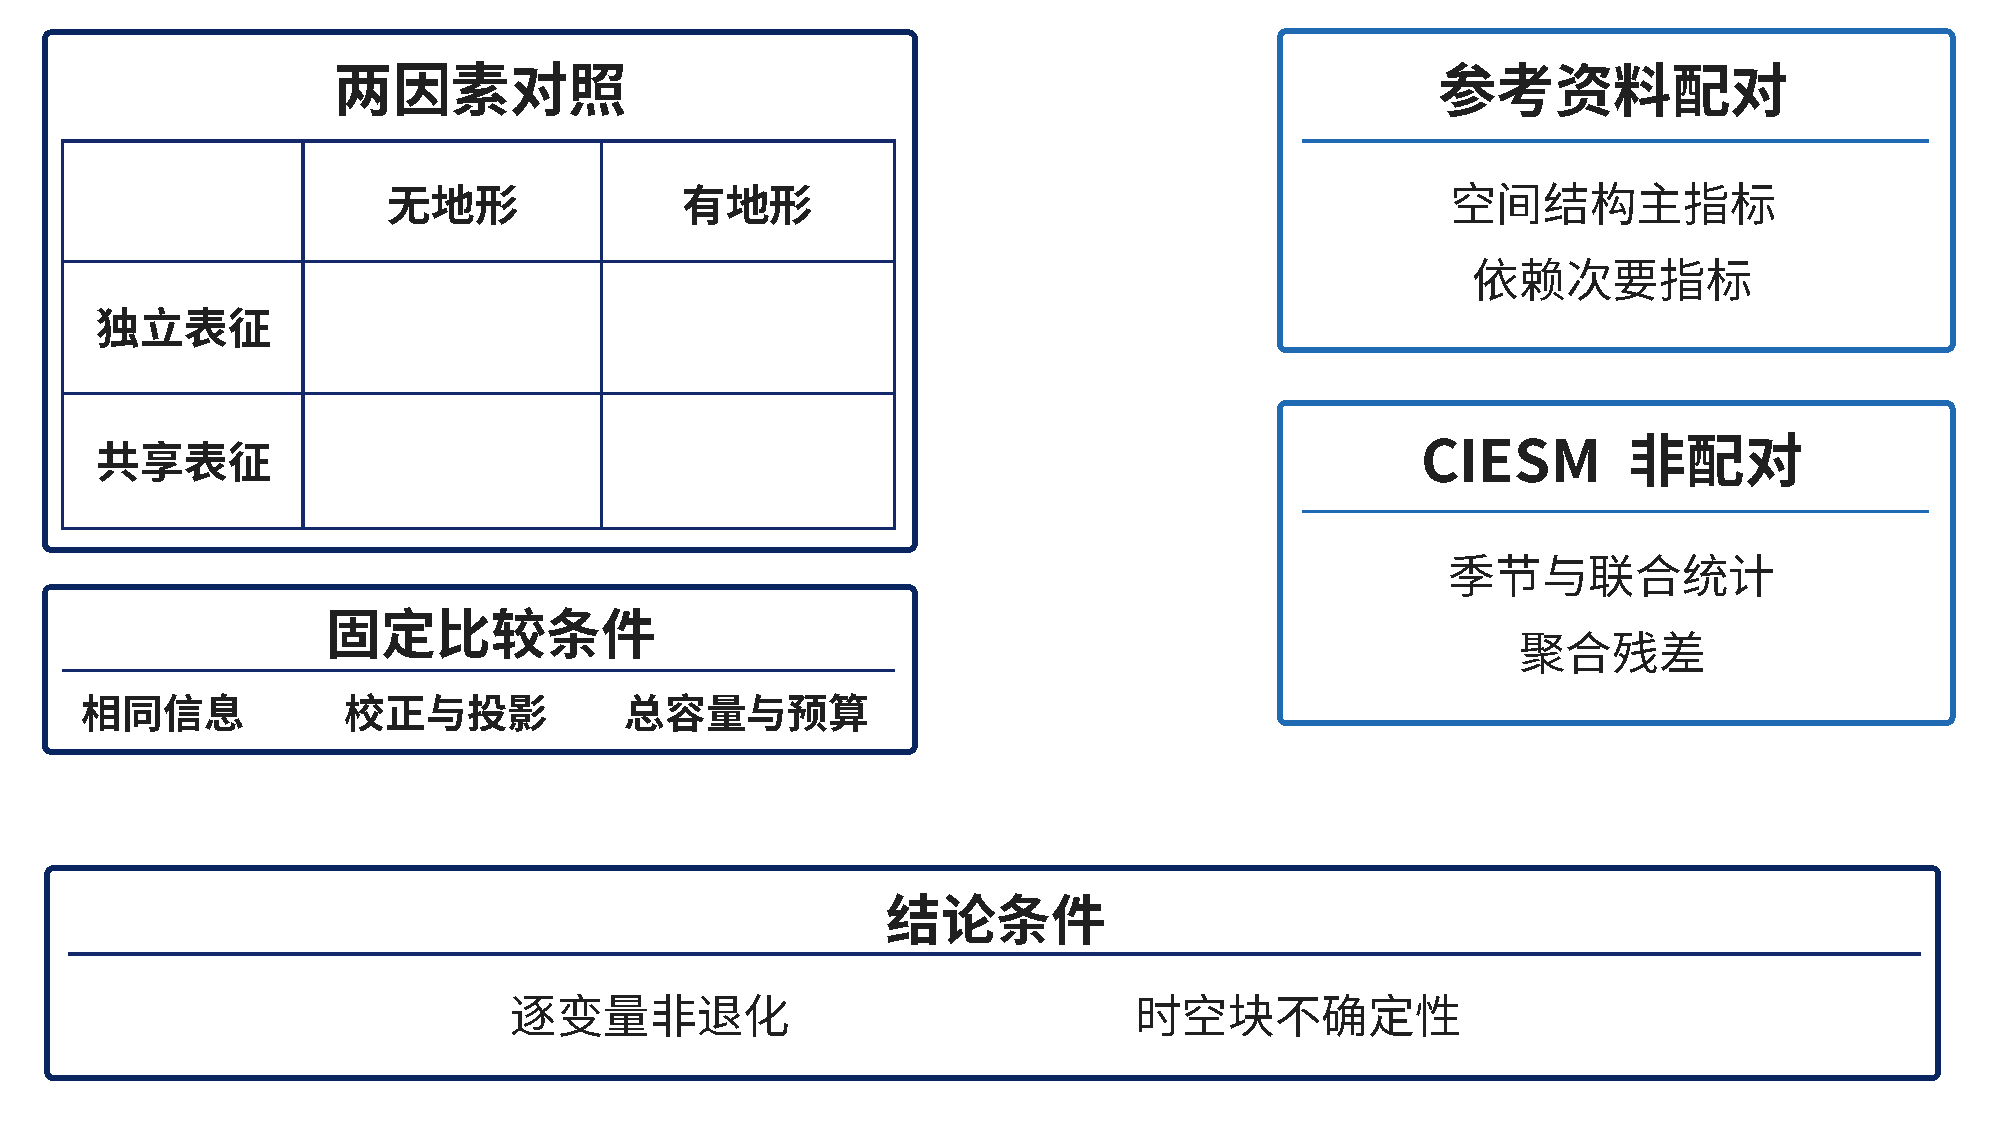
\includegraphics[width=0.95\linewidth]{figures/F07-evaluation.pdf}
\caption{公平消融与两类验证证据。矩阵表示四种拟比较配置；两类资料使用各自评价口径，结论同时检查非退化及不确定性。}
\label{fig:evaluation}
\end{figure}
% NSFC-ILLUSTRATED END F07

